Um circuito integrado foi desenvolvido para avaliar cinco dispositivos APS's, referenciado na se{\c c}\~ao \ref{section:APS} deste documento, e dois TIA's, em refer\^encia \`a se{\c c}\~ao \ref{section:TIA}. O projeto \'e representado em alto n\'ivel na \autoref{fig_circcompleto}. Todos os sinais aqui apresentados na figura, e tamb\'em em todas figuras \'a seguir, seguem o a padr\~o descrito na se{\c c}\~ao \ref{section:padrao_sinais} deste trabalho.

\begin{figure}[htb]
	\caption{\label{fig_circcompleto}Circuito projetado}
	\begin{center}
	    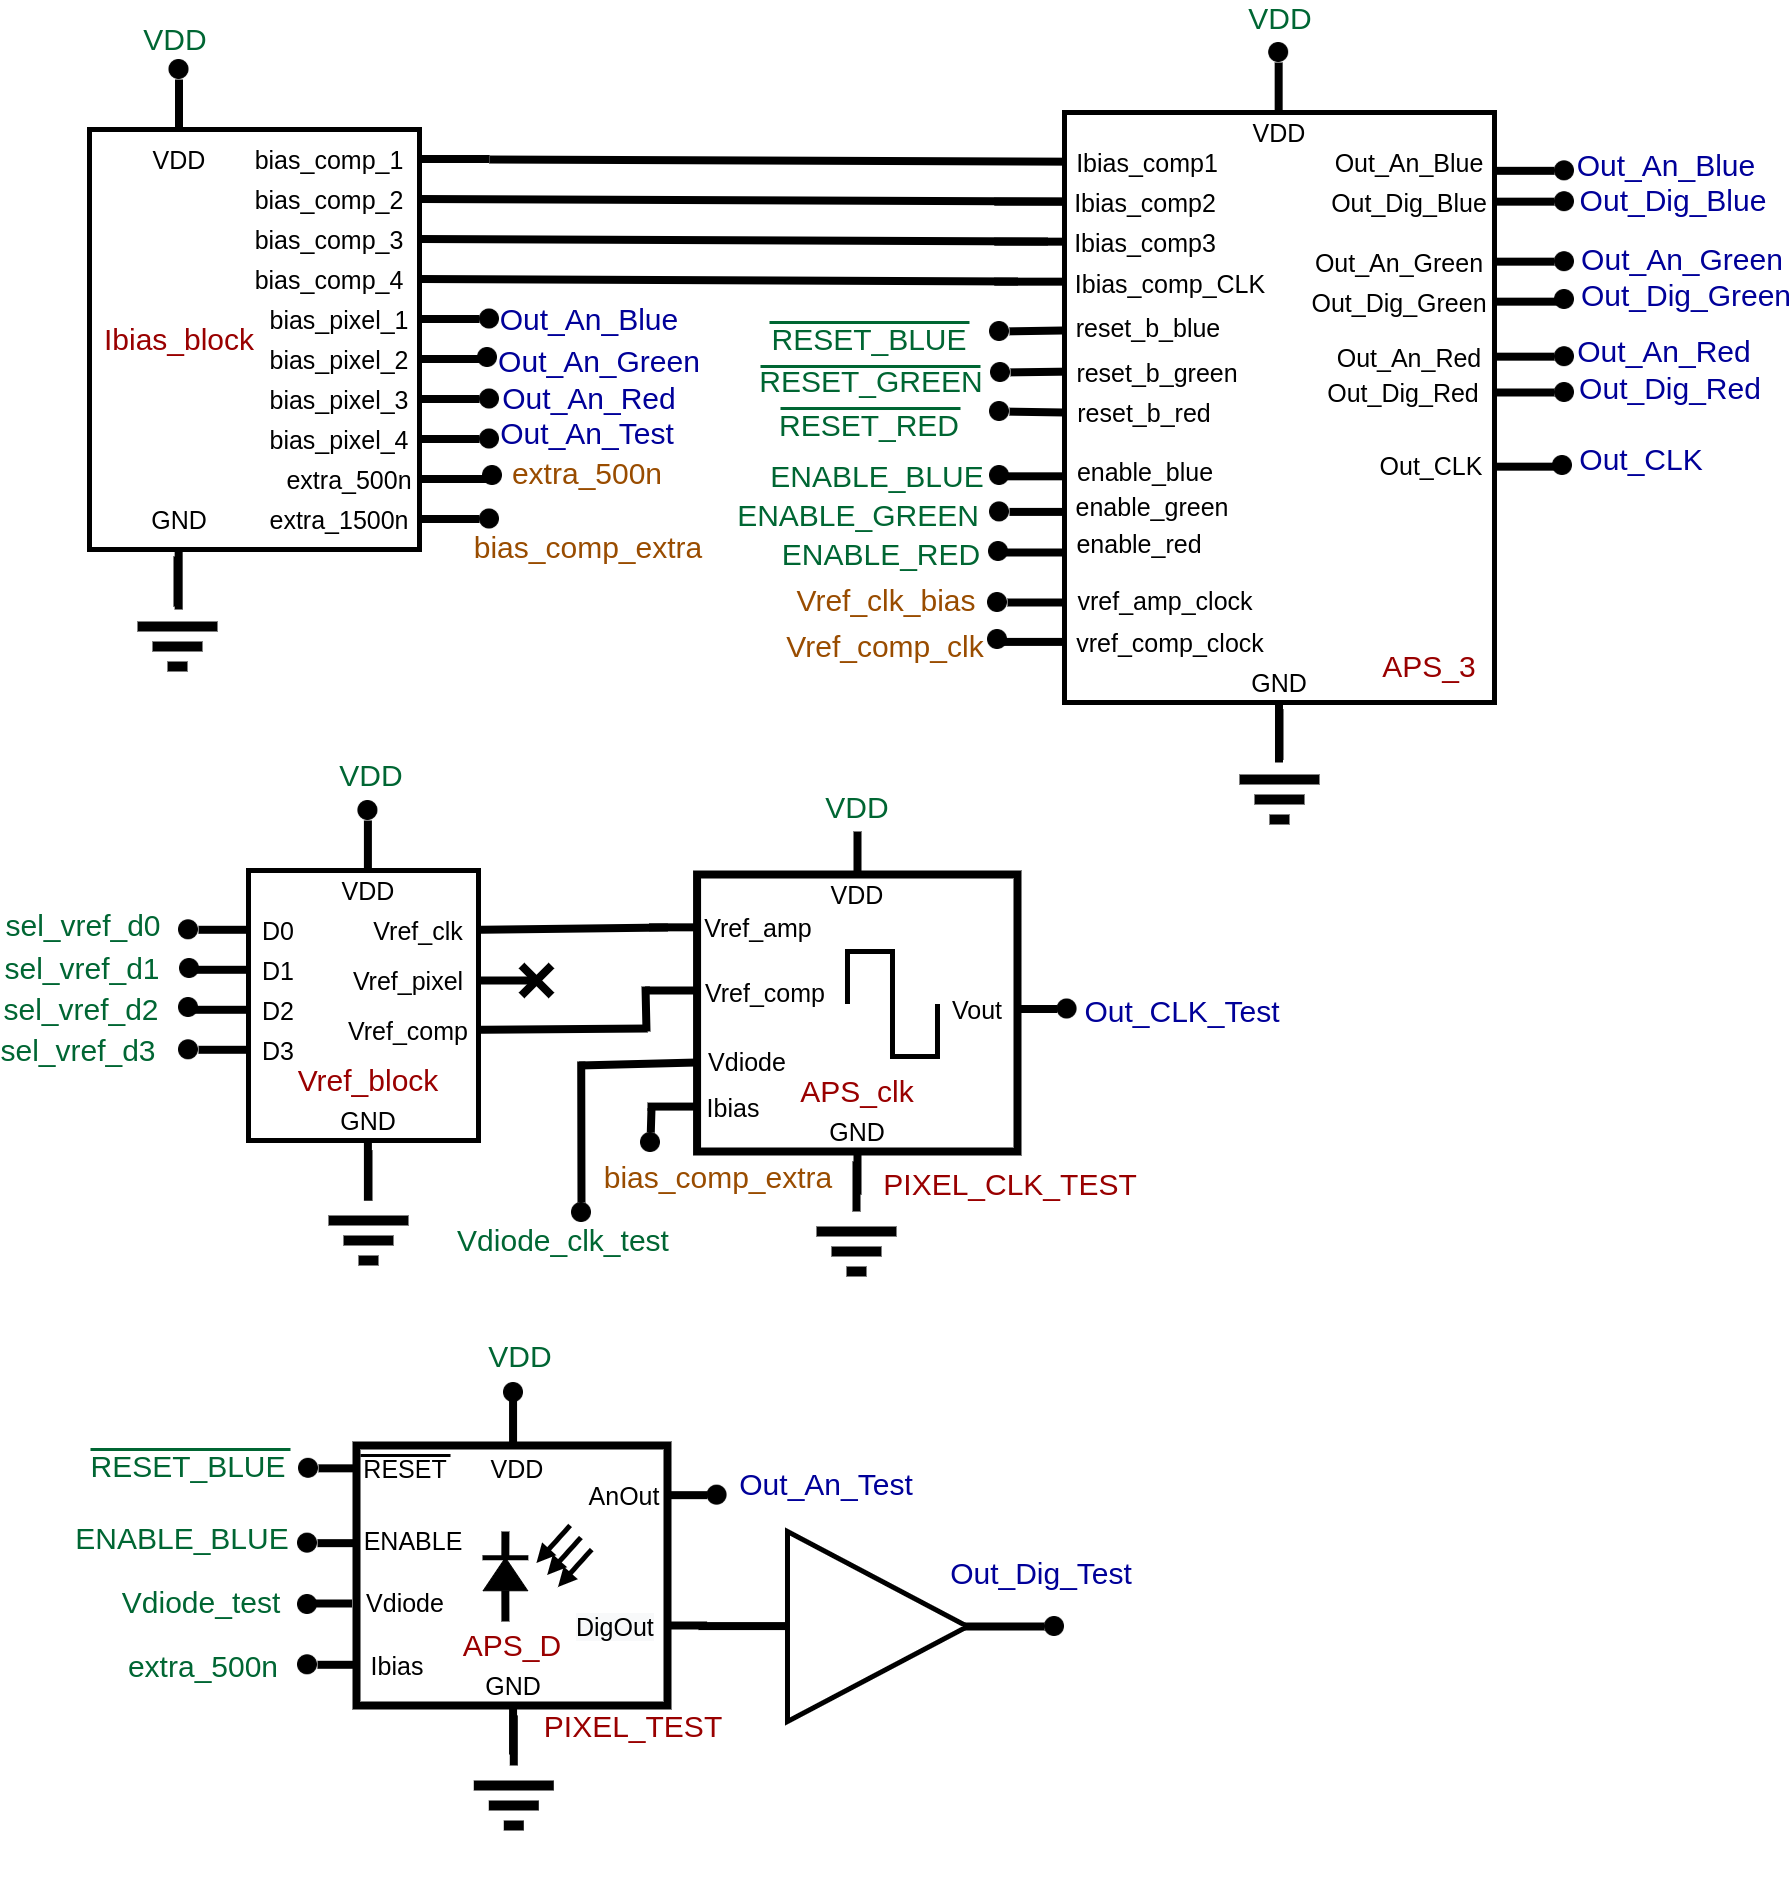
\includegraphics[width=\textwidth]{Circuitos/Complete_Circuit.png}
	\end{center}
	\legend{Fonte: Produzido pelo autor}
\end{figure}

O circuito tem a finalidade de processar a informa{\c c}\~ao advinda de tr\^es APS's, constru\'idos de maneira id\^entica em n\'ivel de layout, com a finalidade de abstrair informa{\c c}\~oes de cores advindas de uma fonte luminosa, dos quais podem ser Azul, Verde ou Vermelha. Para que as cores fossem devidamente separadas entre cada APS, filtros luminosos externo, por meio de uma pel\'icula colorida, s\~ao adicionados sob cada APS respons\'avel por processar uma cor equivalente \`a de sua pel\'icula.

Um sinal luminoso de cor branca tamb\'em \'e utilizado no sistema de forma a ser a refer\^encia de rel\'ogio de todos APS's descritos. Esse sinal \'e processado utilizando-se um $TIA$, do qual \'e gerado um sinal el\'etrico equivalente \'a informa{\c c}\~ao luminosa.

A tecnologia de fabrica{\c c}\~ao utilizada para o desenvolvimento de todos blocos foi a \emph{CMOS 180nm da TSMC}. O software utilizado para o projeto do dispositivo foi o \emph{Virtuoso}, desenvolvido pela \emph{Cadence}.

O circuito representado na \autoref{fig_circcompleto} \'e composto por 2 blocos principais, que permitem o processamento advindos da fonte luminosa, al\'em de um circuito \emph{APS} e um \emph{TIA} extra. A descri{\c c}\~ao dos bloco s\~ao:

\begin{itemize}
    \item \emph{ibias\_block}: Tem a fun{\c c}\~ao de gerar todas fontes de corrente utilizadas em todos os blocos do circuito, quando necess\'ario.
    
    \item \emph{4\_APS}: Implementa os tr\^es circuitos APS descritos, al\'em do circuito \emph{TIA}. A sa\'ida de cada bloco passa por um comparador de forma a digitalizar o dado, como ser\'a melhor explicitado na se{\c c}\~ao \autoref{Bloco4APS}.
    
    \item \emph{Vref\_block} e \emph{PIXEL\_CLK\_TEST}: Estes blocos realizam a implementa{\c c}\~ao de um TIA, por\'em com a adi{\c c}\~ao de um pino extra que possibilita a simula{\c c}\~ao de uma corrente fotogerada sem necessitar de uma fonte luminosa. Estes blocos ser\~ao melhor explicados na se{\c c}\~ao \autoref{BlocoTIA}. 
    
    \item \emph{Vref\_block} e \emph{PIXEL\_TEST}: Este blocos realizam a implementa{\c c}\~ao de um APS, por\'em com a adi{\c c}\~ao de um pino extra que possibilita a simula{\c c}\~ao de uma corrente fotogerada sem necessitar de uma fonte luminosa. Estes blocos ser\~ao melhor explicados na se{\c c}\~ao \autoref{BlocoAPS}.
    
\end{itemize}

A \autoref{tab_circcomp} mostra a rela{\c c}\~ao de sinais de entrada e sa\'ida presentes no circuito, para o processamento dos p\'ixels de cor. A \autoref{tab_circcomp2} mostra a rela{\c c}\~ao de sinais de entrada e sa\'ida presentes no circuito para o processamento dos blocos de teste.

\begin{table}[htb]
\IBGEtab{%
  \caption{Descri{\c c}\~ao dos sinais de entrada e sa\'ida do circuito projetado para as cores azul, verde e vermelha}%
  \label{tab_circcomp}
}{%
  \begin{tabular}{ccll}
  \toprule
   Sinal & Tipo & Descri{\c c}\~ao & Observa{\c c}\~ao \\
  \midrule \midrule
   RESET\_BLUE & Entrada & Sinal de \emph{RESET} no APS para cor azul & Ativo em n\'ivel baixo \\
  \midrule
   RESET\_GREEN & Entrada & Sinal de \emph{RESET} no APS para cor verde & Ativo em n\'ivel baixo \\
  \midrule
   RESET\_RED & Entrada & Sinal de \emph{RESET} no APS para cor vermelha & Ativo em n\'ivel baixo \\
  \midrule
   ENABLE\_BLUE & Entrada & Sinal de \emph{ENABLE} no APS para cor azul & Ativo em n\'ivel alto \\
  \midrule
   ENABLE\_GREEN & Entrada & Sinal de \emph{ENABLE} no APS para cor verde & Ativo em n\'ivel alto \\
  \midrule
   ENABLE\_RED & Entrada & Sinal de \emph{ENABLE} no APS para cor vermelha & Ativo em n\'ivel alto \\
  \midrule
   Out\_An\_Blue & Sa\'ida & Sinal anal\'ogico para cor azul \\
  \midrule
   Out\_Dig\_Blue & Sa\'ida & Sinal digital para cor azul \\
  \midrule
   Out\_An\_Green & Sa\'ida & Sinal anal\'ogico para cor verde \\
  \midrule
   Out\_Dig\_Green & Sa\'ida & Sinal digital para cor verde \\
  \midrule
   Out\_An\_Red & Sa\'ida & Sinal anal\'ogico para cor vermelha \\
  \midrule
   Out\_Dig\_Red & Sa\'ida & Sinal digital para cor vermelha \\
  \bottomrule
\end{tabular}%
}{%
  \fonte{Produzido pelo autor.}
}
\end{table}

\begin{table}[htb]
\IBGEtab{%
  \caption{Descri{\c c}\~ao dos sinais de entrada e sa\'ida do circuito projetado para os blocos de teste}%
  \label{tab_circcomp2}
}{%
  \begin{tabular}{cccc}
  \toprule
   Sinal & Tipo & Descri{\c c}\~ao & Observa{\c c}\~ao \\
  \bottomrule
\end{tabular}%
}{%
  \fonte{Produzido pelo autor.}
}
\end{table}